\section{Decision trees}

\begin{enumerate}
\item Concrete sample training data.
  \begin{enumerate}
  \item The sample entropy $H(Y)$ is $\ldots$.
    \begin{align*}
      H(Y) =&\; \ldots \\
      =&\; \ldots \\
      =&\; \ldots
    \end{align*}

  \item The information gains are $IG(X_1) = \ldots$ and $IG(X_2) = \ldots$.  
    \begin{align*}
      IG(X_1) =&\; \ldots \\
      IG(X_2) =&\; \ldots
    \end{align*}

  \item The decision tree that would be learned is shown in Figure
    \ref{fig:decision_tree}.
    %% The [H], in combination with the float package, forces latex to
    %% generate the figure in exactly this part of the document
    %% instead of ``floating'' it to another part.
    \begin{figure}[H]
      \centering
      \tikzstyle{dir}=[->, very thick]
      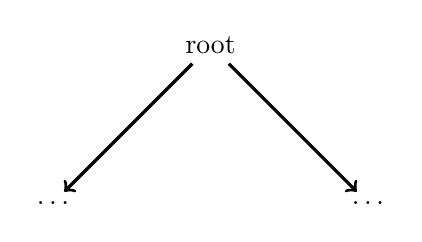
\begin{tikzpicture}[auto]
        \node[rectangle] (root) at (0,0) {root};
        \node (left) at (-2,-2) {$\ldots$};
        \node (right) at (2,-2) {$\ldots$};

        \draw[dir] (root) to [above] node {} (left);
        \draw[dir] (root) to [above] node {} (right);
      \end{tikzpicture}
      \caption{The decision tree that would be learned.}
      \label{fig:decision_tree}
    \end{figure}
  \end{enumerate}

\item Information gain and KL-divergence.
\begin{enumerate}
	\item If variables X and Y are independent, is $IG(x,y) = 0$? If yes, prove it. If no, give a counter example.
	
	\begin{align*}
	IG(x,y)= \ldots \\
	\end{align*}
	
	\item Proof that $IG(x,y) = H[x] - H[x \mid y] = H[y] - H[y \mid x]$,
	starting from the definition in terms of KL-divergence:
	\begin{align*}
	IG(x,y) =&\; KL\left(p(x,y)||p(x)p(y)\right) \\
	=&\; \ldots \\
	=&\; H[x] - H[x \mid y]
	\end{align*}
\end{enumerate}

\end{enumerate}
